% ado file version: 1.3.88
\inserttype[st0001]{article}
\author{S. Kolenikov}{%
  Stanislav Kolenikov\\Abt Associates\\stas\_kolenikov@abtassoc.com
}
\title[Raking survey data: updates]{Updates to the ipfraking ecosystem}
\maketitle

\begin{abstract}
\citet{kolenikov:2014} introduced the package \stcmd{ipfraking}
for iterative proportional fitting (raking) weight calibration procedures
for complex survey designs.
This article briefly describes the original package and updates to the core program,
and documents additional programs that are used to support the process of creating
survey weights in author's production code.

\keywords{\inserttag, survey, calibration, weights, raking}
\end{abstract}

\section{Introduction and background}

Large scale social, behavioral and health data are often collected
via complex survey designs that may involve stratification,
multiple stages of selection and/or unequal probabilities of selection
\citep{korn:graubard:1995,korn:graubard:1999}.
In an ideal setting, varying probabilities of selection are
accounted for by using the Horvitz-Thompson estimator of the totals
\citep{horvitz:thompson:1952,thompson:1997}, and the remaining
sampling fluctuations can be further ironed out by
post-stratification \citep{holt:smith:1979}.
However, on top of the planned differences in probabilities of obtaining
a response from a sampled unit, non-response is a practical problem
that has been growing more acute in recent years
\citep{groves:dillman:eltinge:little:2001,pew:2012}.
The analysis weights that are provided along with the public use
microdata by data collecting agencies are designed to account
for unequal probabilities of selection, non-response, and other factors
affecting imbalance between the population and the sample, thus making
the analyses conducted on such microdata generalizable to the target population.

Earlier work \citep{kolenikov:2014} introduced a Stata package
called \stcmd{ipfraking} that implements
calibration of survey weights to known control totals to ensure
that the resulting weighted data are representative of the population
of interest. The process of calibration is aimed at aligning the sample totals
of the key variables with those known for the population as a whole.
The remainder of this section provides a condensed treatment of estimation
with survey data using calibrated weights; a full description was provided
in the previous paper.

For a given finite population $\mathcal U$ of units indexed $i=1,\ldots,N$,
the interests of survey statisticians often lie in estimating the
population total of a variable $Y$:
\begin{equation}
   T[Y] = \sum_{i \in \mathcal{U}} Y_i
   \label{eq:total:pop}
\end{equation}
A sample $\mathcal S$ of $n$ units indexed by $j=1,\ldots,n$
is taken from $\mathcal U$. If the probability to select the
$i$-th unit is known to be $\pi_i$, then
the {\it probability weights}, or {\it design weights}, are given by
the inverse probability of selection:
\begin{equation}
   w_{di} = \pi_i^{-1}
   \label{eq:prob:weight}
\end{equation}
where subscript $d$ stands for \textit{design} probabilities of selection.
With these weights, an unbiased
(design-based, non-parametric) estimator
of the total (\ref{eq:total:pop}) is \citep{horvitz:thompson:1952}
\begin{equation}
   t[y] = \sum_{j \in \mathcal{S}} \frac{y_j}{\pi_j}
   \equiv \sum_{j \in \mathcal{S}} w_{dj} y_j
   \label{eq:total:sample}
\end{equation}
Probability weights protect
the end user from potentially informative sampling designs, in which
the probabilities of selection are correlated with outcomes, and
relieve the user from the need to fully account for the sampling design
variables in their analysis, as is required in methods such
as multilevel regression with post-stratification \citep{park:gelman:bafumi:2004}.
Design-based methods generally ensure that inference can be generalized
to the finite population even when the statistical models used
by analysts and researchers are not specified correctly
\citep{pfeff:1993,binder:roberts:2003}.

Often, survey statisticians have auxiliary information on the units
in the frame, and such information can be included at the sampling stage
to create more efficient designs. Unequal probabilities of selection
are then controlled with probability weights, implemented
as \stcmd{[pw=}{\it exp}\stcmd{]} in Stata (and can be permanently
affixed to the data set with \stcmd{svyset} command).

In many situations, however, usable information is not available beforehand,
and may only appear in the collected data. For example, the census totals of the age and gender
distribution of the population may exist, but age and gender of
the sampled units is unknown until the survey measurement is taken on them.
It is still possible to capitalize on this additional data by
adjusting the weights in such a way that the reweighted data
conforms to these known figures. The procedures to perform these
reweighting steps are generally known as {\it weight calibration}
\citep{deville:sarndal:1992,deville:sarndal:sautory:1993,%
kott:2006,kott:2009,sarndal:2007}.

Suppose there are several (categorical) variables, referred to
as {\it control variables}, that are available for both
the population and the sample
(age groups, race, gender, educational attainment, etc.).
Weight calibration aims at adjusting the weights
via an iterative optimization
so that the {\it control totals} for the control variables
$\mathbf{x}_j=(x_{1j}, \ldots, x_{pj})$, obtained with the calibrated
weights $w_{cj}$, align with the known population totals:
\begin{equation}
    \sum_{j \in \mathcal{S}} w_{cj} \mathbf{x}_j
    = T [ \mathbf{X}  ]
    \label{eq:control:totals}
\end{equation}
The population totals of the control variables in the right hand side
of (\ref{eq:control:totals}) are assumed to be known from a census or a higher quality survey.
\citet{deville:sarndal:1992} framed the problem of finding a suitable
set of weights as that of constrained optimization with the control
equations (\ref{eq:control:totals}) serving as constraints,
and optimization targeted at making the discrepancy between
the design weights $w_{dj}$ and calibrated weights
$w_{cj}$ as close as possible, in a suitable sense.

The package \stcmd{ipfraking} \citep{kolenikov:2014} implements
a popular calibration algorithm, known as \textit{iterative proportional fitting},
or \textit{raking}, which consists of iterative updating (post-stratification) of
each of the margins. (For an in-depth discussion of distinctions between
raking and post-stratification, see \citet{kolenikov:2016}.)
Since 2014, the continuing code development resulted
in additional features that this update documents.

% REFEREE: COMPARE TO OTHER STATA PACKAGES, OTHER SOFTWARE TOOLS

\section{Updates to \stcmd{ipfraking} program and package}

Listed below is the full syntax of \stcmd{ipfraking}. For description of options,
please refer to \citet{kolenikov:2014}.

\subsection{Syntax of \stcmd{ipfraking}}
\label{subsec:syntax}

\begin{stsyntax}
ipfraking
\optif\
\optin\
\optweight\
,
\underbar{ctot}al({\it matname} [{\it matname \ldots}])
\optional{
\underbar{gen}erate(\newvarname)
replace
double
\underbar{iter}ate(\num)
\underbar{tol}erance(\num)
\underbar{ctrltol}erance(\num)
trace
\underbar{nodiv}ergence
trimhiabs(\num)
trimhirel(\num)
trimloabs(\num)
trimlorel(\num)
trimfrequency(once|sometimes|often)
double
meta
nograph
}
\end{stsyntax}

\subsection{New features of \stcmd{ipfraking}}
\label{subsec:example:meta}

The new features or functionality of \stcmd{ipfraking} concerns reporting and diagnostics;
an alternative functional form specification; and richer metadata stored in the characteristics
of the weight variable.

Reporting of results and errors by \stcmd{ipfraking} was improved in several directions.
\begin{enumerate}
    \item The discrepancy for the worst fitting category is now being reported.
    \item The number of trimmed observations is reported.
    \item If \stcmd{ipfraking} determines that the categories do not match
        in the control totals received from \stcmd{ctotals()} and those found in
        the data, a full listing of categories is provided, and the categories
        not found in one or the other are explicitly shown.
\end{enumerate}

\begin{stlog}
. replace sex_age = 15 if sex_age == 21
(2,056 real changes made)
{\smallskip}
. ipfraking [pw=finalwgt], gen( rakedwgt2d ) ///
>     ctotal( ACS2011_sex_age Census2011_region Census2011_race )
{\smallskip}
categories of sex_age do not match in the control ACS2011_sex_age and in the data
> (nolab option)
This is what ACS2011_sex_age gives:
  _one:11 _one:12 _one:13 _one:21 _one:22 _one:23
This is what I found in data:
  _one:11 _one:12 _one:13 _one:15 _one:22 _one:23
This is what ACS2011_sex_age has that data don't:
  _one:21
This is what data have that ACS2011_sex_age doesn't:
  _one:15
r(111);

\end{stlog}


Linear calibration (Case 1 of \citet{deville:sarndal:1992}) is provided with
\stcmd{linear} option. The weights are calculated analytically:
\begin{equation}
    \label{eq:linear:weight}
    w_{j,\rm{lin}} = w_{dj} (1+\mathbf{x}_j'\mathbf{\lambda}),
    \quad
    \mathbf{\lambda} = \Bigl( \sum_{j \in \mathcal{S}} w_{dj} \mathbf{x}_j \mathbf{x}_j' \Bigr)^{-1}
        ( T [ \mathbf{X}  ] - t[X] )
\end{equation}
Since no iterative optimization is required, linear calibration works very fast.
However it has an undesirable artefact of potentially producing negative weights,
as the range of weights is not controlled. (As raking works by multiplying the currents
weights by positive factors, if the input weights are all positive, the output weights
will be positive as well.) Negative weights are not allowed by the official \stcmd{svy} commands
or commands that work with \stcmd{[pweights]}.
In many tasks, running linear weights first,
pulling up the negative and small positive weights (\stcmd{replace weight = 1 if weight <= 1})
and re-raking using the ``proper'' iterative proportional fitting runs faster than
raking from scratch. An example of linearly calibrated weights is given below
in Section \ref{sec:linear}.

Option \stcmd{meta} saves more information in characteristics of the calibrated
weight variables. Using Example 3 from \citet{kolenikov:2014} with trimming options,
we have:

% TODO: edit the file to trim the output that goes over the right margin

\begin{stlog}
. capture drop rakedwgt3
{\smallskip}
. ipfraking [pw=finalwgt], gen( rakedwgt3 ) ///
>     ctotal( ACS2011_sex_age Census2011_region Census2011_race ) ///
>     trimhiabs(200000) trimloabs(2000) meta
{\smallskip}
\cnp
 Iteration 1, max rel difference of raked weights = 14.95826
\oom
 Iteration 10, max rel difference of raked weights = 2.254e-07
{\smallskip}
   Summary of the weight changes
{\smallskip}
              {\VBAR}    Mean    Std. dev.    Min        Max       CV
\HLI{14}{\PLUS}\HLI{50}
Orig weights  {\VBAR}    11318       7304      2000       79634   .6453
Raked weights {\VBAR}    22055      18908      4033      200000   .8573
Adjust factor {\VBAR}   2.1486               0.9220     18.9828
{\smallskip}
. char li rakedwgt3[]
  rakedwgt3[command]:         [pw=finalwgt], gen( rakedwgt3 ) ctotal( ACS2011_s
> ex_age Ce..
  rakedwgt3[trimloabs]:       trimloabs(2000)
  rakedwgt3[trimhiabs]:       trimhiabs(200000)
  rakedwgt3[trimfrequency]:   sometimes
  rakedwgt3[objfcn]:          2.25435521346e-07
  rakedwgt3[maxctrl]:         3.00266822363e-08
  rakedwgt3[converged]:       1
  rakedwgt3[Census2011_race]: 7.48567503861e-09
  rakedwgt3[Census2011_region]:
                              3.00266822363e-08
  rakedwgt3[ACS2011_sex_age]: 4.13778410340e-09
  rakedwgt3[note1]:           Raking controls used: ACS2011_sex_age Census2011_
> region Ce..
  rakedwgt3[note0]:           1
{\smallskip}
\nullskip
\end{stlog}

The following characteristics are stored with the newly created weight variable
(see \pref{char}).

\noindent
\begin{tabular}{ll}
    \stcmd{command} & The full command as typed by the user \\
    {\it matrix name} & The relative matrix difference from the corresponding \\
                    & control total, see \dref{functions} \\
    \stcmd{trimhiabs}, \stcmd{trimloabs}, & Corresponding trimming options,
                    if specified \\
    \stcmd{trimhirel}, \stcmd{trimlorel}, & \\
    \stcmd{trimfrequency} & \\
    \stcmd{maxctrl} & the greatest \stcmd{mreldif} between the targets and the achieved \\
                    & weighted totals \\
    \stcmd{objfcn}  & the value of the relative weight change at exit \\
    \stcmd{converged} & whether \stcmd{ipfraking} exited due to convergence (1) \\
                    & vs. due to an increase in the objective function \\
                    & or reaching the limit on the number of iterations (0) \\\
    \stcmd{source}  & weight variable specified as the \stcmd{[pw=]} input \\
    \stcmd{worstvar}& the variable in which the greatest discrepancy between \\
                    & the targets and the achieved weighted totals \\
                    & (\stcmd{maxctrl}) was observed \\
    \stcmd{worstcat}& the category of the \stcmd{worstvar} variable in which the  \\
                    & greatest discrepancy was observed
\end{tabular}

For the control total matrices \num$=1,2,\ldots$, the following
meta-information is stored.

\begin{tabular}{ll}
    \stcmd{mat\num} & the name of the control total matrix \\
    \stcmd{totalof\num}& the multiplier variable (matrix \stcmd{coleq}) \\
    \stcmd{over\num}& the margin associated with the matrix \\
                    & (i.e., the categories represented by the columns)
\end{tabular}

Also, \stcmd{ipfraking} stores the notes regarding the control matrices
used, and which of the margins did not match the control totals, if any.
See \dref{notes}.

\subsection{Utility programs}
\label{subsec:utility}

The original package \stcmd{ipfraking} provided additional utility programs:
\stcmd{mat2do}, \stcmd{xls2row} and \stcmd{totalmatrices}.

\subsubsection{Design effects}

A new utility program \stcmd{whatsdeff}
was added to compute the unequal weighting design effects and margins of error, common tasks associated
with describing survey weights. Specifically, the Transparency Initiative
of the American Association for Public Opinion Research
\citep{aapor:2014:ti:terms}
requires that

\begin{quote}
For probability samples, the estimates of sampling error will be reported, and the discussion will state whether or not the reported margins of sampling error or statistical analyses have been adjusted for the design effect due to weighting, clustering, or other factors.
\end{quote}

% \subsubsection{Syntax of \stcmd{whatsdeff}}

\begin{stsyntax}
whatsdeff
{\it weight\_variable}
\optif\
\optin\
,
\optional{
by(\varlist)
}
\end{stsyntax}

The utility program \stcmd{whatsdeff} calculates the apparent design effect due to unequal weighting,
$${\rm DEFF_{UWE}}=1 + {CV}^2_w = \mbox{\stcmd{1 + r(Var)/(r(mean))\^{}2}}$$
using the returned values from \stcmd{summarize} {\it weight{\_}variable} (see \stcmd{help return}).
Additionally, it reports the effective sample size, $n/{\rm DEFF_{UWE}}$, and also returns
the margins of error for the sample proportions that estimate the population proportions of
10\% and 50\%.

\noindent
\begin{stlog}
. webuse nhanes2, clear
{\smallskip}
. whatsdeff finalwgt
{\smallskip}
    Group     {\VBAR}   Min     {\VBAR}   Mean    {\VBAR}   Max     {\VBAR}    CV   {\VBAR}   DEFF  {\VBAR}   N   {\VBAR}  N eff
\HLI{14}{\PLUS}\HLI{11}{\PLUS}\HLI{11}{\PLUS}\HLI{11}{\PLUS}\HLI{9}{\PLUS}\HLI{9}{\PLUS}\HLI{7}{\PLUS}\HLI{8}
      Overall {\VBAR}   2000.00 {\VBAR}  11318.47 {\VBAR}  79634.00 {\VBAR}  0.6453 {\VBAR}  1.4164 {\VBAR} 10351 {\VBAR} 7307.97
{\smallskip}
. return list
{\smallskip}
scalars:
                  r(N) =  10351
              r(MOE10) =  .0068792766212984
              r(MOE50) =  .0114654610354974
       r(Neff_Overall) =  7307.97435325364
       r(DEFF_Overall) =  1.416397964696134
{\smallskip}
. whatsdeff finalwgt, by(sex)
{\smallskip}
    Group     {\VBAR}   Min     {\VBAR}   Mean    {\VBAR}   Max     {\VBAR}    CV   {\VBAR}   DEFF  {\VBAR}   N   {\VBAR}  N eff
\HLI{14}{\PLUS}\HLI{11}{\PLUS}\HLI{11}{\PLUS}\HLI{11}{\PLUS}\HLI{9}{\PLUS}\HLI{9}{\PLUS}\HLI{7}{\PLUS}\HLI{8}
sex           {\VBAR}           {\VBAR}           {\VBAR}           {\VBAR}         {\VBAR}         {\VBAR}       {\VBAR}
         Male {\VBAR}   2000.00 {\VBAR}  11426.14 {\VBAR}  79634.00 {\VBAR}  0.6578 {\VBAR}  1.4326 {\VBAR}  4915 {\VBAR} 3430.94
       Female {\VBAR}   2130.00 {\VBAR}  11221.12 {\VBAR}  61534.00 {\VBAR}  0.6333 {\VBAR}  1.4010 {\VBAR}  5436 {\VBAR} 3880.01
\HLI{14}{\PLUS}\HLI{11}{\PLUS}\HLI{11}{\PLUS}\HLI{11}{\PLUS}\HLI{9}{\PLUS}\HLI{9}{\PLUS}\HLI{7}{\PLUS}\HLI{8}
      Overall {\VBAR}   2000.00 {\VBAR}  11318.47 {\VBAR}  79634.00 {\VBAR}  0.6453 {\VBAR}  1.4164 {\VBAR} 10351 {\VBAR} 7307.97
{\smallskip}
. return list
{\smallskip}
scalars:
                  r(N) =  10351
              r(MOE10) =  .0068792766212984
              r(MOE50) =  .0114654610354974
       r(Neff_Overall) =  7307.97435325364
       r(DEFF_Overall) =  1.416397964696134
        r(Neff_Female) =  3880.00710397866
        r(DEFF_Female) =  1.40102836266093
          r(Neff_Male) =  3430.938195872213
          r(DEFF_Male) =  1.432552765279559
{\smallskip}
\nullskip
\end{stlog}

Design effects can also be broken down by a categorical variable:

\noindent
\begin{stlog}
\input{ipfr.whatsdeff.sex.log.tex}\nullskip
\end{stlog}

% REFEREE:
% 4.	The author should note that whatsdeff produces a design effect due to unequal weighting
% that should be considered as an upper bound on this design effect (a worst case scenario),
% since this calculation assumes that the weights are completely independent of
% the survey variable of descriptive interest.

The estimates of unequal weighting design effects that \stcmd{whatsdeff} produces
should be considered as a typical magnitude of a design effect.
As pointed out by a referee, in many situations when survey variables are correlated with weights
or with the variables that weight calibration is based upon, the actual
design effects reported by postestimation command \stcmd{estat effect} should be expected
to be lower, provided that variance estimation methods take calibration
into account properly (e.g., via replicate variance estimation, as described
in \citet{kolenikov:2010}, or via \stcmd{svy, vce(calibrate)} functionality
of the official Stata \stcmd{svy} suite available in Stata 15.1+).
In other words, for most situations these estimates could be considered an upper bound
on this design effect, since this calculation assumes that the weights are independent of
the survey variable of descriptive interest. Situations can be envisioned, however,
when weighting is counterproductive for efficiency of certain statistics,
e.g., when a group that is oversampled by the sampling design requirements
turns out to have the outcome variance smaller than that of the rest population;
or when screening is applied within rare population sampling designs
\citep{kalton:anderson:1986,kalton:2009}.

\subsubsection{Conversion of the matrices}

One of the utility programs available in \citet{kolenikov:2014}, \stcmd{mat2do},
was updated to provide the \stcmd{notimestamp} option to omit the time stamps
(which tend to unnecessarily throw off the project building and revision control systems).

A new program \stcmd{totalmatrices} converts the control totals matrices between
the formats expected by \stcmd{ipfraking} and \stcmd{svycal}. 

\begin{stsyntax}
totalmatrices
{\it matrix\_list}
,
\optional{
    svycal 
    \underbar{ipfr}aking 
    stub({\it name}) 
    replace
}
\end{stsyntax}

\hangpara
\stcmd{svycal} checks that the supplied matrix or matrices are compatible with \stcmd{svycal} 
specification of totals as a matrix.

\hangpara
\stcmd{ipfraking} checks that the supplied matrix or matrices are compatible with \stcmd{ipfraking}.

\hangpara
\stcmd{stub({\it name})} provides the naming convention for the converted control total matrices.
If the conversion is from \stcmd{ipfraking} to \stcmd{svycal}, one matrix whose name is supplied in 
the \stcmd{stub(...)} option will be created. If the conversion is from \stcmd{svycal} to 
\stcmd{ipfraking}, matrices corresponding to each variable will be created and have their names
set to concatenation of the stub and the variable name.

To convert several matrices from \stcmd{ipfraking} format to a single matrix 
in \stcmd{svycal} format:

\begin{stlog}
\input{ipfr.totalmatrices.log.tex}\nullskip
\end{stlog}

To convert a single matrix compatible with \stcmd{svycal} requirements for its 
\stcmd{totals({\it matname})} format into a list of matrices compatible with
\stcmd{ipfraking}:

\begin{stlog}
. totalmatrices alltotals, ipfraking stub(totmat_) replace convert
It appears that the matrix alltotals is of the svycal format.
Matrices created:
matrix list totmat_sex_age
matrix list totmat_region
matrix list totmat_race
{\smallskip}
. matrix list totmat_region
{\smallskip}
totmat_region[1,4]
            _one:     _one:     _one:     _one:
               1         2         3         4
region  40679030  49205289  85024007  53385843
{\smallskip}
\nullskip
\end{stlog}

Note that at the moment, \stcmd{totalmatrices} does not handle conversion
of interactions, which is arguably one of the greatest strengths of \stcmd{svycal}.
As noted in section \ref{subsec:compare}, for interactions to work out with \stcmd{ipfraking},
standalone variables need to be created, and \stcmd{totalmatrices} would rather
have the user do that.

\subsection{New programs in the package}

Two new programs are added to the package: \stcmd{ipfraking\_report} and \stcmd{wgtcellcollapse},
and are documented in the subsequent sections of this article. The former provides reports on the raked weights,
including summaries of the data with no weights, with the input weights, and with the calibrated weights.
The latter creates a mostly automated flow of collapsing weighting cells that are too detailed
(and hence have low sample sizes).

\section{Excel reports on raked weights:  \stcmd{ipfraking\_report}}

\begin{stsyntax}
ipfraking\_report
using \textit{filename}
,
raked\_weight(\varname)
\optional{
matrices(\textit{namelist})
by(\varlist)
xls
replace
force
}
\end{stsyntax}

The utility command \stcmd{ipfraking\_report} produces a detailed report
describing the raked weights, and places it into \textit{filename}\stcmd{.dta} file
(or, if \stcmd{xls} option is specified, both \textit{filename}\stcmd{.dta} and \textit{filename}\stcmd{.xls}
files).

Along the way, \stcmd{ipfraking\_report} runs a regression of the log raking ratio $w_{3j}/w_{1j}$
on the calibration variables. This regression is expected to have $R^2$ equal to or very close to 1,
and residual variance equal to or very close to zero. This naturally produces obscenely
high $t$-test values, but the purpose of this regression is not in establishing
``significance'' of any variable in explaining the outcome (which we know to be predicted
with near certainty).
Instead, the regression coefficients provide insights regarding which categories received
greater vs. smaller adjustments (which in turn indicate lower response or coverage rates
for the corresponding population subgroups). Conversely, control variables that are
associated with relatively similar adjustment factors may be contributing relatively
little to the weight adjustment, and may be candidates for removal from the list of control totals.

Using the working example from \citet{kolenikov:2014}, the example regression output is:

\begin{stlog}
\input{ipfr.report1.edited.log.tex}\nullskip
\end{stlog}

It looks like \stcmd{ipfraking} had to make greater adjustments to the weights
of older females (\stcmd{sex\_age==23}, i.e., \stcmd{sex==2 \& age==3};
the adjustment factor for this category was 3.732 vs. the low of 1.798 for young women),
and especially other race individuals (the adjustment factor was 9.023,
vs. 1.798 for the whites). The diagnostic value is in the differences in the adjustment
factors with the same variable; since no attempt is being made to average
across the population or the sample or to assign the ``base'' variable,
the absolute reported values of the adjustment factors may not be
meaningful. In the example above, 1.798 figures both as the greatest adjustment
factor of the region variable, and as the lowest adjustment factor
for the race the and sex-by-age interaction. As is easily seen from regression
output, this value is the exponent of the intercept \stcmd{1.798=exp(0.586)}.
Since all of the ``estimates'' of the region specific coefficients are negative,
the lowest reported value is less than this baseline value. Since all of the
``estimates'' of the race and sex-by-age indicators are positive, all
the category-specific adjustment factors are greater than this baseline value.
This is an interplay of the base categories, and the differences in the
demographic composition within each category of a control total variable
vis-a-vis other weighting variables.

\subsection{Options of \stcmd{ipfraking\_report}}

\hangpara
\stcmd{raked\_weight(\varname)} specifies the name of the raked weight variable to create
    the report for. This is a required option.

\hangpara
\stcmd{matrices(\textit{namelist})} specifies a list of matrices (formatted as the matrices
    supplied to \stcmd{ctotal()} option of \stcmd{ipfraking}) to produce weighting reports for.
    In particular, the variables and their categories are picked up from these matrices;
    and the control totals/proportions are compared to those defined by the weight being reported on.

\hangpara
\stcmd{by(\varlist)} specifies a list of additional variables for which the weights are to
    be tabulated in the raking weights report. The difference with the \stcmd{matrices()} option
    is that the control totals for these variables may not be known (or may not be relevant).
    In particular, \stcmd{by(\_one)}, where \stcmd{\_one} is identically one, will produce
    the overall report.

\hangpara
\stcmd{xls} requests exporting the report to an Excel file.

\hangpara
\stcmd{replace} specifies that the files produced by \stcmd{ipfraking\_report} (i.e., the \stcmd{.dta}
    and the {\stmcd{.xls}} file if \stcmd{xls} option is specified) should be overwritten.

\hangpara
\stcmd{force} requires that a variable that may be found repeatedly (between the calibration variables
    supplied originally to \stcmd{ipfraking}, the variables found in the independent total \stcmd{matrices()},
    and the variables without the control totals provided in \stcmd{by()} option) is processed every
    time it is encountered. (Otherwise, it is only processed once.)

\subsection{Variables in the raking report}

The raking report file contains the following variables.

\cnp

\noindent
\begin{tabular}{p{2.25in}p{3.25in}}
  \hline
  Variable name & Definition \\
  \hline
  \stcmd{Weight\_Variable} & The name of the weight variable, \stcmd{generate()} \\
  \stcmd{C\_Total\_Margin\_Variable\_Name} & The name of the control margin, \\
            & \stcmd{rowname} of the corresponding \stcmd{ctotal()} matrix \\
  \stcmd{C\_Total\_Margin\_Variable\_Label} & The label of the control margin variable \\
  \stcmd{Variable\_Class} & The role of the variable in the report: \\
        & Raking margin: a variable used as a calibration margin \\
        & (picked up automatically from the \stcmd{ctotal()} \\
        & matrix, provided \stcmd{meta} option was specified) \\
        & Other known target: supplied with \stcmd{matrices()} \\
        & option of \stcmd{ipfraking\_report} \\
        & Auxiliary variable: additional variable supplied \\
        & with \stcmd{by()} option of \stcmd{ipfraking\_report} \\
%   \hline
% \end{tabular}
%
% \begin{tabular}{p{2.25in}p{3.25in}}
%   \hline
%   Variable name & Definition \\
%   \hline
  \stcmd{C\_Total\_Arg\_Variable\_Name} & The name of the multiplier variable \\
  \stcmd{C\_Total\_Arg\_Variable\_Label} & The label of the multiplier variable \\
  \stcmd{C\_Total\_Margin\_Category\_Number} & Numeric value of the control total category \\
  \stcmd{C\_Total\_Margin\_Category\_Label} &  Label of the control total category \\
  \stcmd{C\_Total\_Margin\_Category\_Cell} & An indicator whether a weighting cell was\\
        & produced by collapsing categories \\
        & using \stcmd{wgtcellcollapse} \\
  \stcmd{Category\_Total\_Target} & The control total to be calibrated to \\
        & (the specific entry in the \stcmd{ctotal()} matrix) \\
  \stcmd{Category\_Total\_Prop} & Control total proportion \\
        & (the ratio of the specific entry in the \stcmd{ctotal()} \\
        & matrix to the matrix total) \\
  \stcmd{Unweighted\_Count} & Number of sample observations in the category \\
  \stcmd{Unweighted\_Prop} & Unweighted proportion \\
  \stcmd{Unweighted\_Prop\_Discrep} & Difference \stcmd{Unweighted\_Prop} - \stcmd{Category\_Total\_Prop} \\
  \stcmd{Category\_Total\_SRCWGT} & Weighted category total, with input weight \\
  \stcmd{Category\_Prop\_SRCWGT} & Weighted category proportion, with input weight \\
  \stcmd{Category\_Total\_Discrep\_SRCWGT} & Difference \stcmd{Category\_Total\_SRCWGT} - \\
        & - \stcmd{Category\_Total\_Target} \\
  \stcmd{Category\_Prop\_Discrep\_SRCWGT} & Difference \stcmd{Category\_Prop\_SRCWGT} - \\
        & - \stcmd{Category\_Total\_Prop} \\
  \stcmd{Category\_RelDiff\_SRCWGT} & \stcmd{reldif(Category\_Total\_SRCWGT,} \\
        & \stcmd{Category\_Total\_Target)} \\
  \stcmd{Overall\_Total\_SRCWGT} & Sum of source weights \\
  \stcmd{Source} & The name of the matrix from which the totals \\
        & were obtained \\
  \stcmd{Comment} & Placeholder for comments, to be entered during \\
        & manual review \\
  \hline
\end{tabular}

For each of the input weights (\stcmd{SRCWGT} suffix), raked weights (\stcmd{RKDWGT} suffix) and raking ratio
(the ratio of raked and input weights, \stcmd{RKDRATIO} suffix), the following summaries are provided.

\begin{tabular}{ll}
  \hline
  Variable name & Definition \\
  \hline
  \stcmd{Min\_\textit{WEIGHT}} & Min of the respective weight \\
  \stcmd{P25\_\textit{WEIGHT}} & 25th percentile of the respective weights \\
  \stcmd{P50\_\textit{WEIGHT}} & Median of the respective weights \\
  \stcmd{P75\_\textit{WEIGHT}} & 75th percentile of the respective weights \\
  \stcmd{Max\_\textit{WEIGHT}} & Max of the respective weights \\
  \stcmd{Mean\_\textit{WEIGHT}} & Mean of the respective weights \\
  \stcmd{SD\_\textit{WEIGHT}} & Standard deviation of the respective weights \\
  \stcmd{DEFF\_\textit{WEIGHT}} & Apparent UWE DEFF of the respective weights \\
  \hline
\end{tabular}

% \clearpage\newpage

\subsection{Example}

Continuing with the example of calibration by region, race, and sex-by-age interaction,
a glimpse of the raking report looks as follows.

\begin{stlog}
. use rakedwgt3-report, clear
(Weighting report on rakedwgt3)
{\smallskip}
. list C_Total_Margin_Variable_Name C_Total_Margin_Category_Label ///
>         Category_Total_Target Category_Total_RKDWGT DEFF_SRCWGT DEFF_RKDWGT , ///
>         sepby( C_Total_Margin_Variable_Name )
{\smallskip}
     {\TLC}\HLI{69}{\TRC}
     {\VBAR} C_Tota..   {\tytilde}y_Label   Categor{\tytilde}t   Categor..   DEFF_SR{\tytilde}T   DEFF_RK{\tytilde}T {\VBAR}
     {\LFTT}\HLI{69}{\RGTT}
  1. {\VBAR}  sex_age         11    41995394    41995394   1.2148059   1.6259899 {\VBAR}
  2. {\VBAR}  sex_age         12    42148662    42148662   1.2462168   1.5716613 {\VBAR}
  3. {\VBAR}  sex_age         13    26515340    26515340   1.2241095   1.5460785 {\VBAR}
  4. {\VBAR}  sex_age         21    41164255    41164255   1.2325105   1.5639529 {\VBAR}
  5. {\VBAR}  sex_age         22    43697440    43697440   1.1937826   1.5175312 {\VBAR}
  6. {\VBAR}  sex_age         23    32773080    32773080    1.233902    1.664307 {\VBAR}
     {\LFTT}\HLI{69}{\RGTT}
  7. {\VBAR}   region         NE    40679030    40679030   1.3056639   1.3657837 {\VBAR}
  8. {\VBAR}   region         MW    49205289    49205289   1.3475551   1.4909581 {\VBAR}
  9. {\VBAR}   region          S    85024007    85024006   1.4950056   1.4912995 {\VBAR}
 10. {\VBAR}   region          W    53385843    53385844    1.459859   2.3772667 {\VBAR}
     {\LFTT}\HLI{69}{\RGTT}
 11. {\VBAR}     race      White   1.784e+08   1.784e+08   1.4059259   1.4337901 {\VBAR}
 12. {\VBAR}     race      Black    29856865    29856865   1.5173846   1.5092533 {\VBAR}
 13. {\VBAR}     race      Other    20053682    20053682   1.3179136   1.2264706 {\VBAR}
     {\LFTT}\HLI{69}{\RGTT}
 14. {\VBAR}     _one          1           .   2.283e+08   1.4164382   1.7349278 {\VBAR}
     {\BLC}\HLI{69}{\BRC}
\nullskip
\end{stlog}

The last line, corresponding to the auxiliary variable \stcmd{\_one} identically
equal to 1 (this variable was present in the data set as it was used by \stcmd{ipfraking}
as a multiplier), contains summaries for the sample as a whole. It is always recommended
to include it (note the use of \stcmd{ipfraking\_report, ... by(\_one)} option
in the syntax in the previous section.)

Functionality of \stcmd{ipfraking\_report} is aimed at manual quality control review,
which typically involves (i) categories with raking factors that differ the most (in the output),
and (ii) the resulting report file in Excel,
although for some aspects of automated quality control, it can be useful, as well.

\section{Collapsing weighting cells:  \stcmd{wgtcellcollapse}}

An additional new component of \stcmd{ipfraking} package is a tool to
semi-automatically collapse weighting cells, in order to achieve
a required minimal size of the weighting cell. (A typical recommendation
is to have cells of size 30 to 50.)

\begin{stsyntax}
wgtcellcollapse \textit{task}
\optif\
\optin\
,
\optional{task\_options}
}
\end{stsyntax}

where \textit{task} is one of:

\hangpara
\stcmd{define} to define collapsing rules explicitly

\hangpara
\stcmd{sequence} to create collapsing rules for a sequence of categories

\hangpara
\stcmd{report} to list the currently defined collapsing rules

\hangpara
\stcmd{candidate} to find rules applicable to a given category

\hangpara
\stcmd{collapse} to perform cell collapsing

\hangpara
\stcmd{label} to label collapsed cells using the original labels after \stcmd{wgtcellcollapse collapse}

\subsection{Syntax of \stcmd{wgtcellcollapse report}}

\begin{stsyntax}
wgtcellcollapse report
,
\underbar{var}iables(\varlist)
\optional{
break
}
\end{stsyntax}

\hangpara
\stcmd{\underbar{var}iables(\varlist)} is the list of variables for which the collapsing rules are to be reported

\hangpara
\stcmd{break} requires \stcmd{wgtcellcollapse report} to exit with error when technical inconsistencies are encountered

\subsection{Syntax of \stcmd{wgtcellcollapse define}}

\begin{stsyntax}
wgtcellcollapse define
,
\underbar{var}iables(\varlist)
\optional{
from(\textit{numlist})
to(\num)
label(\ststring)
max(\num)
clear
}
\end{stsyntax}

\hangpara
\stcmd{\underbar{var}iables(\varlist)} is the list of variables for which the collapsing rule can be used

\hangpara
\stcmd{from(\textit{numlist})} is the list of categories that can be collapsed according to this rule

\hangpara
\stcmd{to(\num)} is the numeric value of the new, collapsed category

\hangpara
\stcmd{label(\ststring)} is the value label to be attached to the new, collapsed category

\hangpara
\stcmd{max(\num)} overrides the automatically determined max value of the collapsed variable

\hangpara
\stcmd{clear} clears all the rules currently defined

\bigskip

Let us demonstrate the two subcommands introduced so far with the following toy example.

\begin{stlog}
{\smallskip}
. 
. clear
{\smallskip}
. 
. set obs 4
number of observations (_N) was 0, now 4
{\smallskip}
. 
. gen byte x = _n
{\smallskip}
. 
. label define x_lbl 1 "One" 2 "Two" 3 "Three" 4 "Four"
{\smallskip}
. 
. label values x x_lbl
{\smallskip}
. 
. wgtcellcollapse define, var(x) from(1 2 3) to(123)
{\smallskip}
. 
. wgtcellcollapse report, var(x)
{\smallskip}
Rule (1): collapse together
  x == 1 (One)
  x == 2 (Two)
  x == 3 (Three)
  into x == 123 (123)
  WARNING: unlabeled value x == 123
{\smallskip}
{\smallskip}
. 
\nullskip
\end{stlog}

For automated quality control purposes, the \stcmd{break} option
of \stcmd{wgtcellcollapse report} can be used to abort the execution
when technical deficiencies in the rules or in the data are encountered.
In the above example, the label of the new category 123 was not defined.
Should the \stcmd{break} option be specified,
this would be considered a serious enough deficiency to stop with an error:

\begin{stlog}
{\smallskip}
. 
. wgtcellcollapse report, var(x) break
{\smallskip}
Rule (1): collapse together
  x == 1 (One)
  x == 2 (Two)
  x == 3 (Three)
  into x == 123 (123)
  ERROR: unlabeled value x == 123
assertion is false
r(9);
{\smallskip}
. 
. wgtcellcollapse define, var(x) clear
{\smallskip}
. 
. wgtcellcollapse define, var(x) from(1 2 3) to(123) label("One through three")
{\smallskip}
. 
. wgtcellcollapse report, var(x) break
{\smallskip}
Rule (1): collapse together
  x == 1 (One)
  x == 2 (Two)
  x == 3 (Three)
  into x == 123 (One through three)
{\smallskip}
{\smallskip}
. 
\nullskip
\end{stlog}

\subsection{Syntax of \stcmd{wgtcellcollapse sequence}}


\begin{stsyntax}
wgtcellcollapse sequence
,
\underbar{var}iables(\varlist)
from(\textit{numlist})
depth(\num)
\end{stsyntax}

\hangpara
\stcmd{\underbar{var}iables(\varlist)} is the list of variables for which the collapsing rule can be used

\hangpara
\stcmd{from(\textit{numlist})} is the sequence of values from which the plausible subsequences can be constructed

\hangpara
\stcmd{depth(\num)} is the maximum number of the original categories that can be collapsed

Continuing with the toy example introduced above, here is an example of moderate length sequences to collapse categories:

\begin{stlog}
. clear
{\smallskip}
. set obs 4
number of observations (_N) was 0, now 4
{\smallskip}
. gen byte x = _n
{\smallskip}
. label define x_lbl 1 "One" 2 "Two" 3 "Three" 4 "Four"
{\smallskip}
. label values x x_lbl
{\smallskip}
. wgtcellcollapse sequence, var(x) from(1 2 3 4) depth(3)
{\smallskip}
. wgtcellcollapse report, var(x)
{\smallskip}
Rule (1): collapse together
  x == 1 (One)
  x == 2 (Two)
  into x == 212 (One to Two)
\cnp
Rule (2): collapse together
  x == 2 (Two)
  x == 3 (Three)
  into x == 223 (Two to Three)
{\smallskip}
Rule (3): collapse together
  x == 3 (Three)
  x == 4 (Four)
  into x == 234 (Three to Four)
{\smallskip}
Rule (4): collapse together
  x == 1 (One)
  x == 2 (Two)
  x == 3 (Three)
  into x == 313 (One to Three)
{\smallskip}
Rule (5): collapse together
  x == 1 (One)
  x == 223 (Two to Three)
  into x == 313 (One to Three)
{\smallskip}
Rule (6): collapse together
  x == 3 (Three)
  x == 212 (One to Two)
  into x == 313 (One to Three)
{\smallskip}
Rule (7): collapse together
  x == 2 (Two)
  x == 3 (Three)
  x == 4 (Four)
  into x == 324 (Two to Four)
{\smallskip}
Rule (8): collapse together
  x == 2 (Two)
  x == 234 (Three to Four)
  into x == 324 (Two to Four)
{\smallskip}
Rule (9): collapse together
  x == 4 (Four)
  x == 223 (Two to Three)
  into x == 324 (Two to Four)
{\smallskip}
\nullskip
\end{stlog}

Note how \stcmd{wgtcellcollapse sequence} automatically created labels for the collapsed cells.

When creating sequential collapses, \stcmd{wgtcellcollapse sequence} uses the following conventions
in creating the new categories:
\begin{itemize}
    \item First comes the length of the collapsed subsequence (up to \stcmd{depth(\num)}).
    \item Then comes the starting value of the category in the subsequence (padded by zeroes as needed).
    \item Then comes the ending value of the category in the subsequence (padded by zeroes as needed).
\end{itemize}

In the example above, rules 7 through 9 lead to collapsing into the new category 324. This
should be interpreted as ``the subsequence of length 3 that starts with category 2 and ends with category 4''.
A numeric value of the collapsed category that reads like 50412 means
``the subsequence of length 5 that starts with category 4 and ends with category 12''.
In that second example, \stcmd{wgtcellcollapse sequence} padded the value of 4 with an additional zero,
so that the length of resulting collapsed category value is always (\stnum of digits of the sequence length) +
twice (\stnum of digits of the greatest source category).

Note that \stcmd{wgtcellcollapse sequence} respects the order in which the categories are
supplied in the \stcmd{from()} option, and does not sort them. If the categories are supplied
in the order 2, 4, 1 and 3, then \stcmd{wgtcellcollapse sequence} would collapse 2 with 4, 4 with 1,
and 1 with 3:

\bigskip

\begin{stlog}
. wgtcellcollapse define, var(x) clear
{\smallskip}
. wgtcellcollapse sequence, var(x) from(2 4 1 3) depth(2)
{\smallskip}
. wgtcellcollapse report, var(x)
{\smallskip}
Rule (1): collapse together
  x == 2 (Two)
  x == 4 (Four)
  into x == 224 (Two to Four)
{\smallskip}
Rule (2): collapse together
  x == 4 (Four)
  x == 1 (One)
  into x == 241 (Four to One)
{\smallskip}
Rule (3): collapse together
  x == 1 (One)
  x == 3 (Three)
  into x == 213 (One to Three)
{\smallskip}
\nullskip
\end{stlog}


\subsection{Syntax of \stcmd{wgtcellcollapse candidate}}

\begin{stsyntax}
wgtcellcollapse candidate
,
\underbar{var}iable(\varname)
category(\num)
\optional{ \max{\num} }
\end{stsyntax}

\hangpara
\stcmd{\underbar{var}iable(\varname)} is the variable whose collapsing rules are to be searched

\hangpara
\stcmd{category(\num)} is the category for which the candidate rules are to be identified

\hangpara
\stcmd{max(\num)} is the maximum value of the categories in the candidate rules to be returned

The rules found are quietly returned through the mechanism of \stcmd{sreturn},
see \pref{return}, as they are intended to stay in memory sufficiently long for
\stcmd{wgtcellcollapse collapse} to evaluate each rule. Going back to the example
from the previous section
with sequential collapses of depth 3, we can identify the following candidates
for categories 2, 212 (collapsed values of 1 and 2), and a non-existent category of 55:

\begin{stlog}
\input{ipfr.collapse4.edited.log.tex}\nullskip
\end{stlog}

In the second call to
the option \stcmd{max(9)} was used to restrict the returned rules to the rules
that deal with the original categories only (so rule 8 that involved a collapsed category 234
was omitted). In the third call, a list of rules
that involve a collapsed category \stcmd{cat(212)} was requested. Requests
for nonexisting categories are not considered errors, but simply produce empty lists
of ``good rules''.

\subsection{Syntax of \stcmd{wgtcellcollapse label}}

\begin{stsyntax}
wgtcellcollapse label
,
\underbar{var}iable(\varname)
\optional{ verbose force }
\end{stsyntax}

\hangpara
\stcmd{\underbar{var}iable(\varname)} is the collapsed variable to be labeled.

\hangpara
\stcmd{verbose} outputs the labeling results. There may be a lot of output.

\hangpara
\stcmd{force} instructs \stcmd{wgtcellcollapse label} to only use categories present in the data.

An example is given in section \ref{subsec:wgtcellcollapse:labels} below.

\subsection{Syntax of \stcmd{wgtcellcollapse collapse}}

\begin{stsyntax}
wgtcellcollapse collapse \optif \optin
,
\underbar{var}iables(\varlist)
mincellsize(\num)
\underbar{sav}ing(\textit{dofile\_name})
\optional{
\underbar{gen}erate(\newvarname)
replace
append
feed(\varname)
strict
sort(\varlist)
run
maxpass(\num)
\underbar{maxcat}egory(\num)
\underbar{zer}oes(\textit{numlist})
greedy
}
\end{stsyntax}

\hangpara
\stcmd{\underbar{var}iables(\varlist)} provides the list of variables whose cells are to be collapsed.
When more than one variable is specified, \stcmd{wgtcellcollapse collapse} proceeds from right to left,
i.e., first attempts to collapse the rightmost variable.

\hangpara
\stcmd{mincellsize(\num)} specifies the minimum cell size for the collapsed cells. For most weighting
purposes, values of 30 to 50 can be recommended.

\hangpara
\stcmd{\underbar{gen}erate(\newvarname)} specifies the name of the collapsed variable to be created.

\hangpara
\stcmd{feed(\varname)} provides the name of an already existing collapsed variable.

\hangpara
\stcmd{strict} modifies the behavior of \stcmd{wgtcellcollapse collapse} so that only
collapsing rules for which all participating categories have nonzero counts are utilized.

\hangpara
\stcmd{sort(\varlist)} sorts the data set before proceeding to collapse the cell.
The default sort order is in terms of the values of the collapsed variable.
A different sort order may produce a different set of collapsed cell when
cells are tied on size.

\hangpara
\stcmd{maxpass(\num)} specifies the maximum number of passes through the data set. The default value is 10000.}

\hangpara
\stcmd{\underbar{maxcat}egory(\num)} is the maximum category value of the variable being collapsed.
It is passed to the internal calls to \stcmd{wgtcellcollapse candidate}, see above.

\hangpara
\stcmd{\underbar{zer}oes(\textit{numlist})} provides a list of the categories of the collapsed
variable that may have zero counts in the data.

\hangpara
\stcmd{greedy} modifies the behavior \stcmd{wgtcellcollapse collapse} to prefer the rules
that collapse the maximum number of categories.

Options to deal with the do-file to write the collapsing code to:	

\hangpara
\stcmd{\underbar{sav}ing(\textit{dofile\_name})} specifies the name of the do-file that will contain the cell collapsing code.

\hangpara
\stcmd{replace} overwrites the do-file if one exists.

\hangpara
\stcmd{append} appends the code to the existing do-file.

\hangpara
\stcmd{run} specifies that the do-file created is run upon completion. This option is typically specified with most runs.

The primary intent of \stcmd{wgtcellcollapse collapse} is to create the code that can be
utilized in both a survey data file and a population targets data file that
are assumed to have identically named variables. Thus it does not only manipulate the data in the memory
and collapses the cells, but also produces the do-file code that can be recycled in automated
weight production.
To that effect, when a do-file is created with the \stcmd{replace} and \stcmd{saving()} options,
the user needs to specify \stcmd{generate()} option to provide the name of the collapsed variable;
and when the said do-file is appended with the the \stcmd{append} and \stcmd{saving()} options,
the name of that variable is provided with the \stcmd{feed()} option.

The algorithm by which \stcmd{wgtcellcollapse collapse} identifies the cells to be collapsed uses
a variation of greedy search.
It first identifies the cells with the lowest (positive) counts; finds the candidate rules
for the variable(s) to be collapsed; evaluates the counts of the collapsed cells across all
these candidate rules; and uses the rule that produces the smallest size of the
collapsed cell across all applicable rules. So when it finds several rules that are applicable
to the cell being currently processed that has a size of 5, and the candidate rules produce cells
of sizes 7, 10 and 15, \stcmd{wgtcellcollapse collapse} will use the rule that produces the cell
of size 7. The algorithm runs until all cells have sizes of at least
\stcmd{mincellsize(\num)} or until \stcmd{maxpass(\num)} passes through the data are executed.
% It is a pretty dumb algorithm, actually, and it fails quite often.
In real world situations with missing data, this basic algorithm often produces inconsistent
results, generally because it fails to identify empty cells, or fully track the cells
that have already been collapsed.
For that reason, a number of options are provided to modify its behavior.
Section \ref{subsec:example} will demonstrate the typical failures, and the ways to overcome them.

\textit{Hint 1}. Since \stcmd{wgtcellcollapse collapse} works with the sample data,
it will not be able to identify categories that are not observed in the sample (e.g., rare categories),
but may be present in the population. This will lead to errors at the raking stage,
when the control total matrices have more categories than the data, forcing \stcmd{ipfraking} to stop.
To help with that, the option \stcmd{zeroes()} allows the user to pass the categories
of the variables that are known to exist in the population but not in the sample.

\textit{Hint 2}. The behavior of \stcmd{wgtcellcollapse collapse, zeroes()} may still not be
satisfactory. As it evaluates the sample sizes of the collapsed cells across a number
of candidate rules that involve zero cells, it may pick up the rule with lowest
number, and that rule may as well leave some other candidate rules with zero cells untouched.
This creates problems when \stcmd{wgtcellcollapse collapse} returns to those untouched cells,
and looks for the existing cells to collapse them with, creating collapsing rules with breaks
in the sequences. To improve upon that behavior, option \stcmd{greedy} makes
\stcmd{wgtcellcollapse collapse} look for a rule that has as many categories as possible, thus collapsing
as many categories with zero counts in one pass as it can.

\textit{Hint 3}. Other than for dealing with zero cells, the option \stcmd{strict} should be specified
most of the time. It effectively makes sure that the candidate rules correspond to the actual data.

\textit{Hint 4}.
If you want to guarantee some specific combination of cells to be collapsed by \stcmd{wgtcellcollapse collapse},
the most reliable way is to explicitly identify them with the \ifexp\ condition, and specify
a very large cell size like \stcmd{mincellsize(10000)} so that \stcmd{wgtcellcollapse collapse} makes every possible
effort to collapse those cells. Since the resulting cell(s) will fall short of that size, the program will exit
with a complaint that this size could not be achieved,
but hopefully the cells will be collapsed as needed.

\textit{Hint 5}.
If any of the cells fail to reach the requires sizes, the problematic value are returned to the user
in the \stcmd{r(failed)} macro as a space delimited list, and in the \stcmd{r(cfailed)}, as a comma-delimited list.
The content of the \stcmd{r(failed)} macro can be used in code that could read

\begin{stlog}
foreach c in `r(failed)' \{
    ...
    * run some diagnostics for each category that failed
    ...
\}
\end{stlog}
while the content of the the \stcmd{r(cfailed)} macro can be used in code that could
read
\begin{stlog}
list ... if inlist(dpston,`r(cfailed)')
\end{stlog}
Also, these returned values should be used in production code by using the \stcmd{assert} command
\citep{gould:2003:tip3} to ascertain that these macros are empty (i.e., no errors
were encountered):
\begin{stlog}
assert "`r(failed)'" == ""
\end{stlog}



\bigskip

A referee noted that \stcmd{wgtcellcollapse} could also have utility in preparing for hotdeck imputation procedures.
The textbook versions of hotdeck procedures impute missing data by assuming a MAR model \citep{rubin:1976}
with conditioning on a set of categorical variables, i.e., cells of a multivariate table. As is in weighting procedures,
hotdeck procedures are more stable with larger cells, so cell collapsing is often recommended to achieve
minimal cell sizes (with an understanding of the bias-vs-variance tradeoff built into these collapsing decisions).
% ADMIT IN THE RESPONSE LETTER THAT I DON'T USE THEM, AND USE MULTIPLE IMPUTATION INSTEAD.
For a review of the hotdeck and related imputation methods, see \citet{andridge:little:2010}.

% TODO: PROMOTE TO A SECTION

\section{Extended motivating example}
\label{subsec:example}

The primary purpose of developing \stcmd{wgtcellcollapse} and adding it to the \stcmd{ipfraking}
suite was to address the need
to collapse cells of the margin variables so that each cell has a minimum sample size;
and to do so in a way that can be easily made consistent between a sample data
and the population targets data. The problem arises when some of the target
variables have dozens of categories, most of which have small counts.
Example where such needs arise include:
\begin{itemize}
    \item transportation surveys, where many stations will have
        low counts of boardings and especially alightings;
    \item country of origin variables in household surveys,
        where most countries will have very low counts;
    \item continuous age variables which can be collapsed into
        age groups differently for the different races.
\end{itemize}
A referee pointed out that an identical problem arises in creating cells
for hot deck imputation procedures \citet{andridge:little:2010}, 
so \stcmd{wgtcellcollapse} could also have utility in that application.

The workflow of \stcmd{wgtcellcollapse} is demonstrated with the following
simulated transportation data set of trips along a commuter metro line composed of 21 stations:

\begin{stlog}
. use stations, clear
{\smallskip}
. list station_id, sep(0)
{\smallskip}
     {\TLC}\HLI{22}{\TRC}
     {\VBAR}           station_id {\VBAR}
     {\LFTT}\HLI{22}{\RGTT}
  1. {\VBAR}           1. Alewife {\VBAR}
  2. {\VBAR}         2. Brookline {\VBAR}
  3. {\VBAR}         8. Carmenton {\VBAR}
  4. {\VBAR}         11. Dogville {\VBAR}
  5. {\VBAR}         18. East End {\VBAR}
  6. {\VBAR}       24. Framington {\VBAR}
  7. {\VBAR}   26. Grand Junction {\VBAR}
  8. {\VBAR}       30. High Point {\VBAR}
  9. {\VBAR}       36. Irvingtown {\VBAR}
 10. {\VBAR}       39. Johnsville {\VBAR}
 11. {\VBAR}      40. King Street {\VBAR}
 12. {\VBAR}         44. Limerick {\VBAR}
 13. {\VBAR}      47. Moscow City {\VBAR}
 14. {\VBAR}     49. Ninth Street {\VBAR}
 15. {\VBAR}     50. Ontario Lake {\VBAR}
 16. {\VBAR} 53. Picadilly Square {\VBAR}
 17. {\VBAR}       55. Queens Zoo {\VBAR}
 18. {\VBAR}   60. Redline Circle {\VBAR}
 19. {\VBAR}    62. Silver Spring {\VBAR}
 20. {\VBAR}      68. Toledo Town {\VBAR}
 21. {\VBAR}    69. Union Station {\VBAR}
     {\BLC}\HLI{22}{\BRC}
\nullskip
\end{stlog}

Suppose turnstile counts were collected at entrances and exits of these stations,
producing the following population figures.

\label{page:station:daypart}

\noindent
\begin{stlog}
. use trip_population, clear
{\smallskip}
. table board_id daypart , c(sum num_pass) cellwidth(10) mi
{\smallskip}
\HLI{21}{\TOPT}\HLI{59}
                     {\VBAR}                          daypart                          
            board_id {\VBAR}    AM Peak      Midday  PM Reverse       Night     Weekend
\HLI{21}{\PLUS}\HLI{59}
          1. Alewife {\VBAR}       1423          34         219         113          44
        2. Brookline {\VBAR}       7198         298         773         169         144
        8. Carmenton {\VBAR}      19254         181        3739         872         422
        11. Dogville {\VBAR}      12626         872        3476         769        1270
        18. East End {\VBAR}       2470         143        1263         145         114
      24. Framington {\VBAR}        634          50        1296         133          60
  26. Grand Junction {\VBAR}       2208         233         439          88         166
      30. High Point {\VBAR}       4319         424        3740         482         115
      36. Irvingtown {\VBAR}       1221          34         444          30         167
      39. Johnsville {\VBAR}         93           4          64           2           6
     40. King Street {\VBAR}        398          46          76          11          13
        44. Limerick {\VBAR}       1021          19         129          53          34
     47. Moscow City {\VBAR}       3300         776         984         140         301
    49. Ninth Street {\VBAR}         38          22         191           5           5
    50. Ontario Lake {\VBAR}        606          22          80          18          23
53. Picadilly Square {\VBAR}        642          71         622         153          69
      55. Queens Zoo {\VBAR}        331          23         174          15          19
  60. Redline Circle {\VBAR}        270           4          63          13           3
   62. Silver Spring {\VBAR}       3402         240         950         206         445
     68. Toledo Town {\VBAR}       5085          61         744         272         112
\HLI{21}{\BOTT}\HLI{59}
{\smallskip}
. table alight_id daypart , c(sum num_pass) cellwidth(10) mi
{\smallskip}
\HLI{21}{\TOPT}\HLI{59}
                     {\VBAR}                          daypart                          
           alight_id {\VBAR}    AM Peak      Midday  PM Reverse       Night     Weekend
\HLI{21}{\PLUS}\HLI{59}
        2. Brookline {\VBAR}         19           .           3           2           .
        8. Carmenton {\VBAR}        492          18          56          23          15
        11. Dogville {\VBAR}       2475          42         423         153          80
        18. East End {\VBAR}        929          31         193          67          68
      24. Framington {\VBAR}        404          13          91          28          27
  26. Grand Junction {\VBAR}        576          20         147          42          41
      30. High Point {\VBAR}       2189          89         560         165         167
      36. Irvingtown {\VBAR}        288          10          91          21          18
      39. Johnsville {\VBAR}         41           .          11           2           1
     40. King Street {\VBAR}        131           3          38           8           6
        44. Limerick {\VBAR}        277           9          87          20          18
     47. Moscow City {\VBAR}       1746          78         556         142         128
    49. Ninth Street {\VBAR}         88           2          25           3           4
    50. Ontario Lake {\VBAR}        232          11          70          14          14
53. Picadilly Square {\VBAR}        633          33         198          47          47
      55. Queens Zoo {\VBAR}        230          10          71          13          14
  60. Redline Circle {\VBAR}         90           2          26           3           4
   62. Silver Spring {\VBAR}       1134          67         369          91          85
     68. Toledo Town {\VBAR}       1372          81         444         112         118
   69. Union Station {\VBAR}      53193        3038       16007        2733        2677
\HLI{21}{\BOTT}\HLI{59}
\nullskip
\end{stlog}

Most people ride the train to the last station, with much smaller traffic at other population centers.

Suppose a survey was administered to a sample of the metro line users, with the following counts
of cases collected.

% \begin{table}

% \caption{Sample frequencies of the trips boardings and alightings. \label{tab:sample:xtab}}

\noindent
\begin{stlog}
. use trip_sample, clear
{\smallskip}
. tab board_id daypart
{\smallskip}
                     {\VBAR}                        daypart
            board_id {\VBAR}   AM Peak     Midday  PM Revers      Night    Weekend {\VBAR}     Total
\HLI{21}{\PLUS}\HLI{55}{\PLUS}\HLI{10}
          1. Alewife {\VBAR}        46          4         11          7          3 {\VBAR}        71 
        2. Brookline {\VBAR}       236          4         35          6          7 {\VBAR}       288 
        8. Carmenton {\VBAR}       653          4        184         47         24 {\VBAR}       912 
        11. Dogville {\VBAR}       410         41        166         35         56 {\VBAR}       708 
        18. East End {\VBAR}        85          5         64          4          4 {\VBAR}       162 
      24. Framington {\VBAR}        30          3         74          3          1 {\VBAR}       111 
  26. Grand Junction {\VBAR}        72         13         23          5          6 {\VBAR}       119 
      30. High Point {\VBAR}       158         20        187         25         12 {\VBAR}       402 
      36. Irvingtown {\VBAR}        34          2         25          1         15 {\VBAR}        77 
      39. Johnsville {\VBAR}         5          1          1          0          0 {\VBAR}         7 
     40. King Street {\VBAR}        17          1          2          0          1 {\VBAR}        21 
        44. Limerick {\VBAR}        28          0          9          1          3 {\VBAR}        41 
     47. Moscow City {\VBAR}        94         31         49          7         13 {\VBAR}       194 
    49. Ninth Street {\VBAR}         0          0          9          0          0 {\VBAR}         9 
    50. Ontario Lake {\VBAR}        13          1          4          1          1 {\VBAR}        20 
53. Picadilly Square {\VBAR}        23          4         35          7          5 {\VBAR}        74 
      55. Queens Zoo {\VBAR}        10          1         14          0          2 {\VBAR}        27 
  60. Redline Circle {\VBAR}        13          0          5          0          0 {\VBAR}        18 
   62. Silver Spring {\VBAR}       106         18         38         12         17 {\VBAR}       191 
     68. Toledo Town {\VBAR}       149          6         33         11          3 {\VBAR}       202 
\HLI{21}{\PLUS}\HLI{55}{\PLUS}\HLI{10}
               Total {\VBAR}     2,182        159        968        172        173 {\VBAR}     3,654 
{\smallskip}
{\smallskip}
. tab alight_id daypart
{\smallskip}
                     {\VBAR}                        daypart
           alight_id {\VBAR}   AM Peak     Midday  PM Revers      Night    Weekend {\VBAR}     Total
\HLI{21}{\PLUS}\HLI{55}{\PLUS}\HLI{10}
        2. Brookline {\VBAR}         1          0          0          0          0 {\VBAR}         1 
        8. Carmenton {\VBAR}        11          1          1          0          1 {\VBAR}        14 
        11. Dogville {\VBAR}        85          1         14          6          5 {\VBAR}       111 
        18. East End {\VBAR}        36          1         18          1          4 {\VBAR}        60 
      24. Framington {\VBAR}        15          1          2          2          2 {\VBAR}        22 
  26. Grand Junction {\VBAR}        15          2          8          1          1 {\VBAR}        27 
      30. High Point {\VBAR}        73          4         22         11          8 {\VBAR}       118 
      36. Irvingtown {\VBAR}         9          0          4          2          2 {\VBAR}        17 
      39. Johnsville {\VBAR}         3          0          1          0          0 {\VBAR}         4 
     40. King Street {\VBAR}         0          0          3          0          0 {\VBAR}         3 
        44. Limerick {\VBAR}        13          0          2          0          2 {\VBAR}        17 
     47. Moscow City {\VBAR}        81          6         22          6          6 {\VBAR}       121 
    49. Ninth Street {\VBAR}         3          1          1          0          0 {\VBAR}         5 
    50. Ontario Lake {\VBAR}         2          0          1          2          1 {\VBAR}         6 
53. Picadilly Square {\VBAR}        23          1          8          3          2 {\VBAR}        37 
      55. Queens Zoo {\VBAR}         6          0          5          1          0 {\VBAR}        12 
  60. Redline Circle {\VBAR}         5          0          0          0          0 {\VBAR}         5 
   62. Silver Spring {\VBAR}        49          0         19          3          9 {\VBAR}        80 
     68. Toledo Town {\VBAR}        43          3         24          6          7 {\VBAR}        83 
   69. Union Station {\VBAR}     1,709        138        813        128        123 {\VBAR}     2,911 
\HLI{21}{\PLUS}\HLI{55}{\PLUS}\HLI{10}
               Total {\VBAR}     2,182        159        968        172        173 {\VBAR}     3,654 
{\smallskip}
{\smallskip}
\nullskip
\end{stlog}

% \end{table}

As only \input{sample.size.tex}\nullskip surveys were collected from a total of
\input{pop.size.tex}\nullskip riders, we would reasonably expect that there is a need
for weighting and nonresponse adjustment.
The data available for calibration includes the population turnstile counts
listed above. We will produce interactions of the day part and the station that will serve as two
weighting margins (one for the stations where the metro users boarded, and one for the stations
where they got off).

First, we need to define the weighting rules. In this case, the stations are numbered sequentially,
with the northernmost, say, station Alewife being number 3, and the southernmost station,
Union Station, where everybody gets off to rush to their city jobs or attractions, being number 69.
Below, we create a list of stations and provide it to \stcmd{wgtcellcollapse sequence}.
We would be collapsing stations along the line, with the expectation that travelers boarding or leaving
at adjacent stations within the same day part are more similar to one another than the travelers
boarding or leaving a particular station at different times of the day. Collapsing rules
need to be defined for the \stcmd{daypart} variable as well --- mostly because \stcmd{wgtcellcollapse collapse}
expects all variables to have collapsing rules defined.

\begin{stlog}
. use trip_sample, clear
{\smallskip}
. wgtcellcollapse sequence , var(daypart) from(2 3 4) depth(3)
{\smallskip}
. levelsof board_id, local(stations_on)
3 6 10 13 17 21 25 28 32 36 39 42 46 49 52 56 59 63 66 70
{\smallskip}
. levelsof alight_id, local(stations_off)
6 10 13 17 21 25 28 32 36 39 42 46 49 52 56 59 63 66 70 73
{\smallskip}
. local all_stations : list stations_on | stations_off
{\smallskip}
. wgtcellcollapse sequence , var(board_id alight_id) from(`all_stations') depth(20)
{\smallskip}
\nullskip
\end{stlog}

The syntax above relies on the stations being in the sequential order, which is how
the output of \stcmd{levelsof} is organized. Otherwise, the internal numeric identifiers of the stations
would need to be supplied in the order in which the trains run through them.

The number of collapsing rules for variables \stcmd{board\_id} and \stcmd{alight\_id}
created by \stcmd{wgtcellcollapse sequence}
is \input{station.nrules.tex}\nullskip each.

Below we present the final syntax to produce the collapsed cells. 
A more detailed version of the paper, available upon request from the author,
describes the process of building the syntax through trial and (mostly) error.
A reader who plans to thoroughly utilize \stcmd{wgtcellcollapse} should
read the full description.


\begin{stlog}
. use trip_sample_rules, clear
{\smallskip}
. wgtcellcollapse collapse, variables(daypart board_id) mincellsize(1) ///
>         zeroes(39 44 49 60) greedy maxcategory(99) ///
>         generate(dpston5) saving(dpston5.do) replace run
Pass 0 through the data...
  smallest count = 1 in the cell      2000039
{\smallskip}
Processing zero cells...
{\smallskip}
  Invoking rule 49:50=24950 to collapse zero cells
  replace dpston5 = 1024950 if inlist(dpston5, 1000049, 1000050)
Pass 0 through the data...
  smallest count = 1 in the cell      2000039
  Invoking rule 40:44=24044 to collapse zero cells
  replace dpston5 = 2024044 if inlist(dpston5, 2000040, 2000044)
Pass 0 through the data...
  smallest count = 1 in the cell      2000039
  Invoking rule 49:50=24950 to collapse zero cells
  replace dpston5 = 2024950 if inlist(dpston5, 2000049, 2000050)
\smallskip
\oom
\smallskip
Pass 0 through the data...
  smallest count = 1 in the cell      2000039
  Invoking rule 55:60=25560 to collapse zero cells
  replace dpston5 = 5025560 if inlist(dpston5, 5000055, 5000060)
Pass 0 through the data...
  smallest count = 1 in the cell      2000039
Pass 10 through the data...
  smallest count = 1 in the cell      2000039
  Done collapsing! Exiting...
{\smallskip}
. wgtcellcollapse collapse, variables(daypart board_id) mincellsize(20) ///
>         strict feed(dpston5) saving(dpston5.do) append run
Pass 10 through the data...
  smallest count = 1 in the cell      2000039
  Invoking rule 39:24044=33944
  replace dpston5 = 2033944 if inlist(dpston5, 2000039, 2024044)
Pass 11 through the data...
  smallest count = 1 in the cell      2024950
  Invoking rule 53:24950=34953
  replace dpston5 = 2034953 if inlist(dpston5, 2000053, 2024950)
\smallskip
\oom
\smallskip
Pass 55 through the data...
  smallest count = 19 in the cell      3025560
  Invoking rule 62:25560=35562
  replace dpston5 = 3035562 if inlist(dpston5, 3000062, 3025560)
Pass 56 through the data...
  smallest count = 20 in the cell      5026268
  Done collapsing! Exiting...
{\smallskip}
. assert "`r(failed)'" == ""
{\smallskip}
. wgtcellcollapse collapse, variables(daypart alight_id) mincellsize(1) ///
>         zeroes(2 40 60) greedy maxcategory(99) ///
>         generate(dpstoff5) saving(dpstoff5.do) replace run
Pass 0 through the data...
  smallest count = 1 in the cell      1000002
{\smallskip}
Processing zero cells...
{\smallskip}
  Invoking rule 39:40=23940 to collapse zero cells
  replace dpstoff5 = 1023940 if inlist(dpstoff5, 1000039, 1000040)
Pass 0 through the data...
  smallest count = 1 in the cell      1000002
  Invoking rule 1:2:8=30108 to collapse zero cells
  replace dpstoff5 = 2030108 if inlist(dpstoff5, 2000001, 2000002, 2000008)
Pass 0 through the data...
  smallest count = 1 in the cell      1000002
  Invoking rule 30:36:39:40:44=53044 to collapse zero cells
  replace dpstoff5 = 2053044 if inlist(dpstoff5, 2000030, 2000036, 2000039, 2000040,
>  2000044)
\smallskip
\oom
\smallskip
Pass 0 through the data...
  smallest count = 1 in the cell      1000002
  Invoking rule 53:55:60=35360 to collapse zero cells
  replace dpstoff5 = 5035360 if inlist(dpstoff5, 5000053, 5000055, 5000060)
Pass 0 through the data...
  smallest count = 1 in the cell      1000002
Pass 12 through the data...
  smallest count = 1 in the cell      1000002
  Done collapsing! Exiting...
{\smallskip}
. wgtcellcollapse collapse if inlist(daypart,4,5) \& inrange(alight_id,49,50), ///
>         variables(daypart alight_id) mincellsize(1) ///
>         feed(dpstoff5) zeroes(49) maxcategory(99) saving(dpstoff5.do) append run
Pass 12 through the data...
  smallest count = 1 in the cell      1000002
{\smallskip}
Processing zero cells...
{\smallskip}
  Invoking rule 49:50=24950 to collapse zero cells
  replace dpstoff5 = 4024950 if inlist(dpstoff5, 4000049, 4000050)
Pass 12 through the data...
  smallest count = 1 in the cell      1000002
  Invoking rule 49:50=24950 to collapse zero cells
  replace dpstoff5 = 5024950 if inlist(dpstoff5, 5000049, 5000050)
Pass 12 through the data...
  smallest count = 1 in the cell      1000002
Pass 14 through the data...
  smallest count = 1 in the cell      5024950
  Done collapsing! Exiting...
{\smallskip}
. * special cells for weekend
. wgtcellcollapse collapse if daypart==5 \& inrange(alight_id,1,36), ///
>         variables(daypart alight_id) mincellsize(50) ///
>         strict feed(dpstoff5) saving(dpstoff5.do) append run
Pass 14 through the data...
  smallest count = 1 in the cell      5000026
  Invoking rule 24:26=22426
  replace dpstoff5 = 5022426 if inlist(dpstoff5, 5000024, 5000026)
Pass 15 through the data...
  smallest count = 1 in the cell      5030108
  Invoking rule 11:30108=40111
  replace dpstoff5 = 5040111 if inlist(dpstoff5, 5000011, 5030108)
Pass 16 through the data...
  smallest count = 2 in the cell      5033640
  Invoking rule 30:33640=43040
  replace dpstoff5 = 5043040 if inlist(dpstoff5, 5000030, 5033640)
Pass 17 through the data...
  smallest count = 3 in the cell      5022426
  Invoking rule 18:22426=31826
  replace dpstoff5 = 5031826 if inlist(dpstoff5, 5000018, 5022426)
Pass 18 through the data...
  smallest count = 6 in the cell      5040111
  Invoking rule 40111:31826=70126
  replace dpstoff5 = 5070126 if inlist(dpstoff5, 5040111, 5031826)
Pass 19 through the data...
  smallest count = 10 in the cell      5043040
  Invoking rule 70126:43040=110140
  replace dpstoff5 = 5110140 if inlist(dpstoff5, 5070126, 5043040)
Pass 20 through the data...
  smallest count = 23 in the cell      5110140
  WARNING: could not find any rules to collapse dpstoff5 == 5110140
Pass 21 through the data...
  smallest count = .i in the cell      1000002
  Done collapsing! Exiting...
{\smallskip}
\cnp
. wgtcellcollapse collapse if daypart==5 \& inrange(alight_id,44,68), ///
>         variables(daypart alight_id) mincellsize(50) ///
>         strict feed(dpstoff5) saving(dpstoff5.do) append run
Pass 20 through the data...
  smallest count = 1 in the cell      5024950
  Invoking rule 24950:35360=54960
  replace dpstoff5 = 5054960 if inlist(dpstoff5, 5024950, 5035360)
Pass 21 through the data...
  smallest count = 2 in the cell      5000044
  Invoking rule 44:47=24447
  replace dpstoff5 = 5024447 if inlist(dpstoff5, 5000044, 5000047)
Pass 22 through the data...
  smallest count = 3 in the cell      5054960
  Invoking rule 24447:54960=74460
  replace dpstoff5 = 5074460 if inlist(dpstoff5, 5024447, 5054960)
Pass 23 through the data...
  smallest count = 7 in the cell      5000068
  Invoking rule 62:68=26268
  replace dpstoff5 = 5026268 if inlist(dpstoff5, 5000062, 5000068)
Pass 24 through the data...
  smallest count = 11 in the cell      5074460
  Invoking rule 74460:26268=94468
  replace dpstoff5 = 5094468 if inlist(dpstoff5, 5074460, 5026268)
Pass 25 through the data...
  smallest count = 27 in the cell      5094468
  WARNING: could not find any rules to collapse dpstoff5 == 5094468
Pass 26 through the data...
  smallest count = .i in the cell      1000002
  Done collapsing! Exiting...
{\smallskip}
. * all other cells
. wgtcellcollapse collapse, variables(daypart alight_id) mincellsize(20) ///
>         strict feed(dpstoff5) saving(dpstoff5.do) append run
Pass 25 through the data...
  smallest count = 1 in the cell      1000002
  Invoking rule 2:8=20208
  replace dpstoff5 = 1020208 if inlist(dpstoff5, 1000002, 1000008)
Pass 26 through the data...
  smallest count = 1 in the cell      2000011
  Invoking rule 11:18=21118
  replace dpstoff5 = 2021118 if inlist(dpstoff5, 2000011, 2000018)
\smallskip
\oom
\smallskip
Pass 64 through the data...
  smallest count = 15 in the cell      3054960
  Invoking rule 62:54960=64962
  replace dpstoff5 = 3064962 if inlist(dpstoff5, 3000062, 3054960)
Pass 65 through the data...
  smallest count = 21 in the cell      2200168
  Done collapsing! Exiting...
{\smallskip}
. assert "`r(failed)'" == ""
{\smallskip}
\nullskip
\end{stlog}

The resulting cells satisfy the sample size requirements of at least 20 cases per cell:

\begin{stlog}
. bysort dpston5:  assert _N >= 20
\smallskip
. bysort dpstoff5: assert _N >= 20
\end{stlog}

The do-files created by \stcmd{wgtcellcollapse} (see the \stcmd{saving(...)} option) 
can now be applied to producing control totals, and eventually to raking:

\begin{stlog}
. use trip_population, clear
{\smallskip}
. run dpston5.do
{\smallskip}
. total num_pass , over(dpston5)
{\smallskip}
Total estimation                  Number of obs   =        719
{\smallskip}
      1000001: dpston5 = 1000001
      1000002: dpston5 = 1000002
\smallskip
\oom
\smallskip
      5000011: dpston5 = 5000011
      5026268: dpston5 = 5026268
      5030108: dpston5 = 5030108
      5051836: dpston5 = 5051836
      5093960: dpston5 = 5093960
{\smallskip}
\HLI{13}{\TOPT}\HLI{48}
        Over {\VBAR}      Total   Std. Err.     [95\% Conf. Interval]
\HLI{13}{\PLUS}\HLI{48}
num_pass     {\VBAR}
     1000001 {\VBAR}       1423   967.7508     -476.9595    3322.959
     1000002 {\VBAR}       7198    4895.91     -2414.011    16810.01
\smallskip
\oom
\smallskip
     5000011 {\VBAR}       1270    834.301      -367.961    2907.961
     5026268 {\VBAR}        557   364.4324     -158.4805    1272.481
     5030108 {\VBAR}        610   263.2061      93.25444    1126.746
     5051836 {\VBAR}        622   215.5712      198.7749    1045.225
     5093960 {\VBAR}        473   261.8954     -41.17225    987.1723
\HLI{13}{\BOTT}\HLI{48}
{\smallskip}
. matrix dpston5 = e(b)
{\smallskip}
. matrix coleq dpston5 = _one
{\smallskip}
. matrix rownames dpston5 = dpston5
{\smallskip}
. run dpstoff5.do
{\smallskip}
. total num_pass , over(dpstoff5)
{\smallskip}
Total estimation                  Number of obs   =        719
{\smallskip}
      1000018: dpstoff5 = 1000018
      1000030: dpstoff5 = 1000030
\smallskip
\oom
\smallskip
      5000069: dpstoff5 = 5000069
      5094468: dpstoff5 = 5094468
      5110140: dpstoff5 = 5110140
{\smallskip}
\HLI{13}{\TOPT}\HLI{48}
        Over {\VBAR}      Total   Std. Err.     [95\% Conf. Interval]
\HLI{13}{\PLUS}\HLI{48}
num_pass     {\VBAR}
     1000018 {\VBAR}        929   360.7303      220.7878    1637.212
     1000030 {\VBAR}       2189   868.0319      484.8161    3893.184
\smallskip
\oom
\smallskip
     5000069 {\VBAR}       2677   895.7917       918.316    4435.684
     5094468 {\VBAR}        432   87.57763      260.0612    603.9388
     5110140 {\VBAR}        423   120.0254      187.3574    658.6426
\HLI{13}{\BOTT}\HLI{48}
{\smallskip}
. matrix dpstoff5 = e(b)
{\smallskip}
. matrix coleq dpstoff5 = _one
{\smallskip}
. matrix rownames dpstoff5 = dpstoff5
{\smallskip}
. use trip_sample_rules, clear
{\smallskip}
. run dpston5
{\smallskip}
. run dpstoff5
{\smallskip}
. gen byte _one = 1
{\smallskip}
. ipfraking [pw=_one], ctotal(dpston5 dpstoff5) gen(raked_weight5)
{\smallskip}
 Iteration 1, max rel difference of raked weights = 37.856256
 Iteration 2, max rel difference of raked weights = .06404821
 Iteration 3, max rel difference of raked weights = .00891802
 Iteration 4, max rel difference of raked weights = .00128619
 Iteration 5, max rel difference of raked weights = .00018966
 Iteration 6, max rel difference of raked weights = .00002818
 Iteration 7, max rel difference of raked weights = 4.198e-06
 Iteration 8, max rel difference of raked weights = 6.257e-07
The worst relative discrepancy of  7.8e-08 is observed for dpstoff5 == 5110140
Target value =        423; achieved value =        423
{\smallskip}
   Summary of the weight changes
{\smallskip}
              {\VBAR}    Mean    Std. dev.    Min        Max       CV
\HLI{14}{\PLUS}\HLI{50}
Orig weights  {\VBAR}        1          0         1           1       0
Raked weights {\VBAR}   26.487      5.754    13.174      38.634   .2172
Adjust factor {\VBAR}  26.4869              13.1743     38.6339
{\smallskip}
. whatsdeff raked_weight5
{\smallskip}
  Group   {\VBAR}   Min     {\VBAR}   Mean    {\VBAR}   Max     {\VBAR}    CV   {\VBAR}   DEFF  {\VBAR}   N   {\VBAR}  N eff
\HLI{10}{\PLUS}\HLI{11}{\PLUS}\HLI{11}{\PLUS}\HLI{11}{\PLUS}\HLI{9}{\PLUS}\HLI{9}{\PLUS}\HLI{7}{\PLUS}\HLI{8}
  Overall {\VBAR}     13.17 {\VBAR}     26.49 {\VBAR}     38.63 {\VBAR}  0.2172 {\VBAR}  1.0472 {\VBAR}  3654 {\VBAR} 3489.37
{\smallskip}
\nullskip
\end{stlog}

Each pass identified the smallest cell count, the cell where this low count is found,
the rule that can be used to collapse this cell with some other cell (see more on determination
of what \stcmd{wgtcellcollapse} believes to be the best rule below), and Stata code
that can be used to apply this collapsing rule.

The collapsed values of the variables \stcmd{dpston} (DayPart-STation-ON) and
\stcmd{dpstoff} (DayPart-STation-OFF) combine the values of the parent variables. The value
of \stcmd{dpston==1000003} indicates the combination of categories
\stcmd{daypart==1} and station number 3.
\label{page:dpston:nomenclature}
The value of \stcmd{dpston==1023940} indicates
\stcmd{daypart==1} and sequence of two stations from 39 to 40.
The value of \stcmd{dpston==2053044} indicates \stcmd{daypart==2} and sequence of
five stations from 30 to 44.

The first call to \stcmd{wgtcellcollapse} uses the options \stcmd{generate()}
and \stcmd{replace} to create a new variable and a new do-file,
while subsequent calls \stcmd{feed()} this variable back, and \stcmd{append} additional
cell collapsing code to the existing do-file.

The \stcmd{zeroes()} options of \stcmd{wgtcellcollapse collapse} provides
notified \stcmd{wgtcellcollapse} that there are values of \stcmd{alight\_id} that 
are never observed. (Riders get on the train on these stations, and exit in small numbers;
but no completed surveys were obtained.)
The \stcmd{mincellsize(1)} option effectively instructed \stcmd{wgtcellcollapse} to exit
once all of these zero cells are identified. The \stcmd{maxcategory(99)} option
restricts collapsing rules to only those that involve individual stations 
(since all the individual station IDs are less than 99, and all of the collapsed values
are at least \stcmd{20102} (i.e., the first two stations merged together, forming 
a cell of size \stcmd{2} that stretched from \stcmd{01} to \stcmd{02}). Without these options,
\stcmd{wgtcellcollapse} would be allowed to pick up one of the previously collapsed cells.
It seems safer to collapse stations with zero count to only one station though.

The use of the subsampling conditions \stcmd{if daypart==5 & inrange(alight\_id,1,36)}
effectively specifies one specific collapsing cell that the algorithm could not otherwise 
identify. A higher target value \stcmd{mincellsize(50)} is used in conjunction, to make
sure that the algorithm does not exit prematurely.
The special missing value \stcmd{.i} that appears in the smallest count report is
used internally to stop \stcmd{wgtcellcollapse} after all of the relevant cases
selected by the \ifexp\ conditions have been processed.

The use of \stcmd{greedy} option made it possible to collapse the streak
of zero counts in the mid-day part from \stcmd{36. Irvington} to \stcmd{44. Limerick}.
Without it, each individual zero count station would be paired with a non-missing station,
which leads to cells that overlap in space. These are clearly unsatisfactory.

After all zero counts stations are processed, the \stcmd{strict} option should almost
always be specified. It prevents \stcmd{wgtcellcollapse} from picking up rules that
may have skipped categories in them. In other words, it ensures that the collapsed cells are 
contiguous.

As its output, \stcmd{wgtcellcollapse} produced two files, one for each
weighting margin, called \stcmd{dpston.do} and \stcmd{dpstoff.do}. An interested reader
is welcome to \stcmd{list} them; they contain long sequences of \stcmd{replace}
commands to perform the cell collapsing. These do-files
are run on the population data to create identical collapsed categories and produce
the matrices of the population control totals for \stcmd{ipfraking}.


\subsection{Informative labels}
\label{subsec:wgtcellcollapse:labels}

Once the collapsing rules are finalized, several types of category labels can be attached to the resulting
collapsed cells.
Using the mechanics of labels in multiple languages (see \rref{label language}),
\stcmd{wgtcellcollapse label} defines three
``languages'' to describe the cells. The language \stcmd{numbered\_ccells} may be convenient
for debugging purposes in fine-tuning the collapsing algorithms, while the language
\stcmd{texted\_ccells} would prove useful for \stcmd{ipfraking\_report} in creating human-readable
labels. (In Stata SMCL output, the \stcmd{label language} instructions are clickable,
so the user does not have to copy and paste the command, but can click it instead.)

\begin{stlog}
. wgtcellcollapse label, var(dpston5) 
(language default renamed unlabeled_ccells)
(language numbered_ccells now current language)
(language texted_ccells now current language)
{\smallskip}
To attach the numeric labels (of the kind "dpston5==1000001"), type:
   label language numbered_ccells
To attach the text labels (of the kind "dpston5==AM Peak; 1. Alewife"), type:
   label language texted_ccells
The original state, which is also the current state, is:
   label language unlabeled_ccells
{\smallskip}
{\smallskip}
. wgtcellcollapse label, var(dpstoff5) 
{\smallskip}
To attach the numeric labels (of the kind "dpstoff5==1000018"), type:
   label language numbered_ccells
To attach the text labels (of the kind "dpstoff5==AM Peak; 18. East End"), type:
   label language texted_ccells
The original state, which is also the current state, is:
   label language unlabeled_ccells
{\smallskip}
{\smallskip}
. label language numbered_ccells
{\smallskip}
. tab dpstoff5 if daypart==5
{\smallskip}
   Long ID of the interaction {\VBAR}      Freq.     Percent        Cum.
\HLI{30}{\PLUS}\HLI{35}
    daypart==5, alight_id==69 {\VBAR}        123       71.10       71.10
 daypart==5, alight_id==94468 {\VBAR}         27       15.61       86.71
daypart==5, alight_id==110140 {\VBAR}         23       13.29      100.00
\HLI{30}{\PLUS}\HLI{35}
                        Total {\VBAR}        173      100.00
{\smallskip}
. label language texted_ccells
{\smallskip}
. tab dpstoff5 if daypart==5
{\smallskip}
             Long ID of the interaction {\VBAR}      Freq.     Percent        Cum.
\HLI{40}{\PLUS}\HLI{35}
             Weekend; 69. Union Station {\VBAR}        123       71.10       71.10
Weekend; 44. Limerick to 68. Toledo Tow {\VBAR}         27       15.61       86.71
 Weekend; 1. Alewife to 40. King Street {\VBAR}         23       13.29      100.00
\HLI{40}{\PLUS}\HLI{35}
                                  Total {\VBAR}        173      100.00
{\smallskip}
. label language unlabeled_ccells
{\smallskip}
. tab dpstoff5 if daypart==5
{\smallskip}
Interaction {\VBAR}
       s of {\VBAR}
    daypart {\VBAR}
 alight_id, {\VBAR}
  with some {\VBAR}
 collapsing {\VBAR}      Freq.     Percent        Cum.
\HLI{12}{\PLUS}\HLI{35}
    5000069 {\VBAR}        123       71.10       71.10
    5094468 {\VBAR}         27       15.61       86.71
    5110140 {\VBAR}         23       13.29      100.00
\HLI{12}{\PLUS}\HLI{35}
      Total {\VBAR}        173      100.00
{\smallskip}
\nullskip
\end{stlog}


\section{Linear calibrated weights}
\label{sec:linear}

Using the final set of collapsed categories in the simulated transportation data example,
let us demonstrate the linear calibration option of
\stcmd{ipfraking}, added since \citet{kolenikov:2014}. In mathematical terms,
linear weights explicitly solve the minimization problem of finding a set of weights
$\{ w_{li}, i=1,\ldots,n \}$, where the subscript $l$ stands for \textit{linear} calibration, such that
\begin{equation}
  \sum_{i=1}^n \frac{(w_{li} - w_{di})^2}{w_{di}} \to \min
  \label{eq:linear:weights}
\end{equation}
\citet{deville:sarndal:1992} and \citet{sarndal:swens:wret:1992} provide
explicit treatment of the problem and the resulting analytical expressions
coded in \stcmd{ipfraking, linear}.
The main advantage of linear weight calibration is a much faster computing time.
To demonstrate it, we will time the output by using
the immediate timing results, \stcmd{set rmsg on} (see \rref{set}).
% REFEREE:
% Please add more description of the results in Figure 1. What is the user to infer from this plot?
% What should users do if this plot takes on other appearances (i.e., there are more discrepancies
% between the two adjusted weights)?

\bigskip

\begin{stlog}
. cap drop raked_weight5*
{\smallskip}
. set rmsg on
r; t=0.00 14:59:22
{\smallskip}
. ipfraking [pw=_one], ctotal(dpston5 dpstoff5) nograph gen(raked_weight5)
{\smallskip}
 Iteration 1, max rel difference of raked weights = 37.856256
 Iteration 2, max rel difference of raked weights = .06404821
 Iteration 3, max rel difference of raked weights = .00891802
 Iteration 4, max rel difference of raked weights = .00128619
 Iteration 5, max rel difference of raked weights = .00018966
 Iteration 6, max rel difference of raked weights = .00002818
 Iteration 7, max rel difference of raked weights = 4.198e-06
 Iteration 8, max rel difference of raked weights = 6.257e-07
The worst relative discrepancy of  7.8e-08 is observed for dpstoff5 == 5110140     
Target value =        423; achieved value =        423
{\smallskip}
   Summary of the weight changes
{\smallskip}
              {\VBAR}    Mean    Std. dev.    Min        Max       CV
\HLI{14}{\PLUS}\HLI{50} 
Orig weights  {\VBAR}        1          0         1           1       0
Raked weights {\VBAR}   26.487      5.754    13.174      38.634   .2172
Adjust factor {\VBAR}  26.4869              13.1743     38.6339
r; t=2.16 14:59:24
{\smallskip}
. ipfraking [pw=_one], ctotal(dpston5 dpstoff5) nograph gen(raked_weight5l) linear
{\smallskip}
Linear calibration
The worst relative discrepancy of  1.8e-14 is observed for dpstoff5 == 5110140     
Target value =        423; achieved value =        423
{\smallskip}
   Summary of the weight changes
{\smallskip}
              {\VBAR}    Mean    Std. dev.    Min        Max       CV
\HLI{14}{\PLUS}\HLI{50} 
Orig weights  {\VBAR}        1          0         1           1       0
Raked weights {\VBAR}   26.487     5.7523    12.518      38.204   .2172
Adjust factor {\VBAR}  26.4869              12.5178     38.2040
r; t=0.63 14:59:25
{\smallskip}
. set rmsg off
{\smallskip}
. label variable raked_weight5l "Linear calibrated weights"
{\smallskip}
. compare raked_weight5 raked_weight5l
{\smallskip}
                                        \HLI{10} difference \HLI{10}
                            count       minimum      average     maximum
\HLI{72}
raked_w{\tytilde}5<raked_{\tytilde}5l          1896     -1.813144    -.0476911   -3.11e-11
raked_w{\tytilde}5>raked_{\tytilde}5l          1758      2.18e-09     .0514348    2.405758
                       \HLI{10}
jointly defined              3654     -1.813144     3.21e-10    2.405758
                       \HLI{10}
total                        3654
{\smallskip}
\nullskip
\end{stlog}

\begin{figure}[hb!]
    \begin{center}
    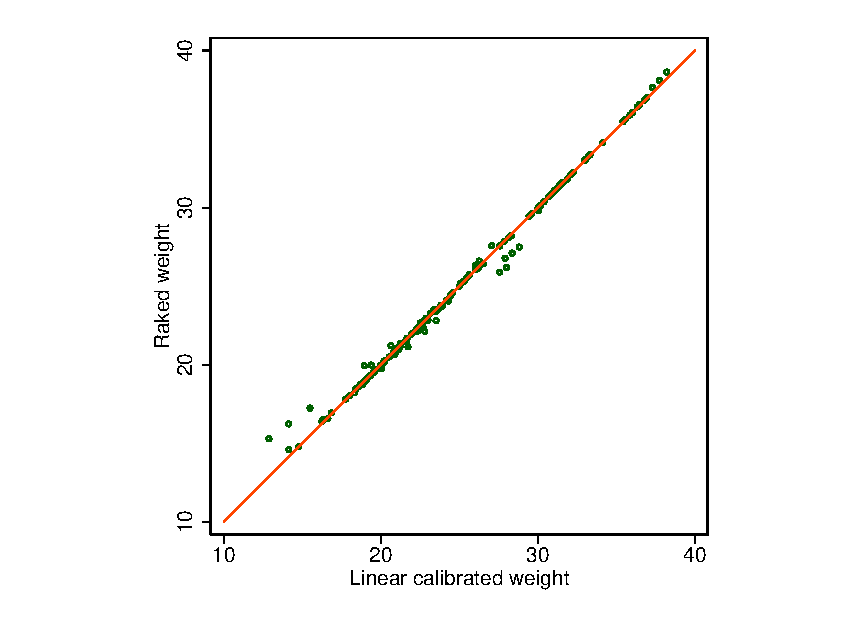
\epsfig{file=raked_linear,width=320}
    \end{center}
    \caption{Linear and raked weights}
    \label{fig:linear:raked}
\end{figure}

\clearpage

The speed advantages of \stcmd{linear} calibration are quite clear (0.63 seconds vs. 2.16 seconds),
even though raking convergence in 8 iterations is quite fast, in author's experience.
It is not unusual to see dozens iterations, and when higher order interactions are being used as
raking margins, subtle correlations between the cells arise, slowing down convergence and requiring
hundreds of iterations.
% TODO: time/profile better -- most of the time is spent in parsing
Linear calibrated and raked weights are very similar to one another, as Figure \ref{fig:linear:raked}
demonstrates, albeit the lowest of the linearly
calibrated weights are slightly smaller than comparable raked weights.
As the two methods are distinct, the weights should be expected to agree in general,
but the match along the diagonal line of the plot should not be expected to be ideal.

As mentioned before, in the extreme situations, linearly calibrated weights
may become negative, which creates additional issues.  First, Stata's \stcmd{svy}
commands or estimation commands with \stcmd{pweight} specifications do not accept
negative weights, and produce error messages when such weights are encountered.
(This is not a bug, but indeed a welcome behavior.) Second, negative weights are
typically difficult to interpret; within a common, although not technically accurate,
interpretation of sampling weights as the number of population units that a sampled
unit represents, it is puzzling to find a negative number of such population units.
The way the author uses the linear calibration functionality of \stcmd{ipfraking}
is to produce ``preliminary'' sets of weights. If the weights at the low end
satisfy the natural range restriction (greater than 0, so as not to produce
input data check errors with estimation commands; or sometimes greater than 1,
so as to satisfy the ``number of population units'' interpretation that is often
desirable for the clinets), these weights can be ``accepted'' as final. If they do not,
\stcmd{ipfraking} can be called with trimming syntax such as \stcmd{trimloabs(1)}.
The linear weights can then be used as a starting point to accelerate convergence.

% TODO: create an example where this is an issue, show the workaround
% See if this is internalized properly by svy calibrate linear.

While the general theory of calibrated estimation \citep{deville:sarndal:1992}
ensures that linear calibrated weights (analyzed as Case 1 in that paper) and
raked weights (Case 2) are asymptotically equivalent, this equivalence implicitly
requires that the scales of the population control matrices are identical.
In practice, different control total variables may come from different sources,
and some sources may have either different populations to which they can technically
be generalized, or come at different scales such as proportions vs. population totals.
Nearly every general population dual frame RDD survey that the present author had dealt
with would use the American Community Survey data for demographic variables
(that would come with the desirable population scaling), and National Health Interview Survey
data for phone use variables (cell phone only, landline only, both, or none) that would
come in the form of proportions. While the raking version of \stcmd{ipfraking} would not
have any difficulty incorporating both (with the caveat that the final scale of weights
will be determined by the \textit{last} variable in the \stcmd{ctotal()} list),
the linear version of weights would try to find a middle point between the population
totals that are on the scale of millions, and proportions that are on the scale of about 1.
The results would likely be quite strange.

\section{Other packages with similar functionality}
\label{subsec:compare}

There exist other packages that provide similar basic functionality
(i.e., raked weights without trimming).
\citet{kolenikov:2014} provided comparisons with
\stcmd{survwgt} \citep{winter:2002}, \stcmd{ipfweight} \citep{bergmann:2011},
\stcmd{maxentropy} \citep{wittenberg:2010}, and reported that the weights
produced by these packages were identical within numeric accuracy.

Yet another weight calibration
package that was published simultaneously with \citet{kolenikov:2014}
was \stcmd{sreweight} \citep{pacifico:2014}. It implements a full range
of objective functions from \citet{deville:sarndal:1992}, and does so faster
than \stcmd{ipfraking} as the core iterative functionality is implemented in Mata.
% Describe what Pacifico does
Finally, Stata 15.1 now provides \stcmd{svycal} command,
undocumented at the time of the writing of this paper, although described
and exemplified in detail in \citet{valliant:dever:2017}. Compared
to \stcmd{svycal}, the core functionality of \stcmd{ipfraking} provides
a richer set of trimming specifications. The author compared the weights
produced by \stcmd{ipfraking} with those produced by \stcmd{sreweight}
and \stcmd{svycal}
in the case of basic raking procedure without trimming, and they agree within
numeric accuracy:

\begin{stlog}
. svycal rake ibn.sex_age ibn.region ibn.race [pw=finalwgt], ///
>         generate(rakedwgt2a) totals(alltotals) nocons
note: 4.region omitted because of collinearity
note: 3.race omitted because of collinearity
{\smallskip}
. compare rakedwgt2 rakedwgt2a
{\smallskip}
                                        \HLI{10} difference \HLI{10}
                            count       minimum      average     maximum
\HLI{72}
rakedwgt2<rakedw{\tytilde}2a          6843     -.0057653    -.0001227   -3.27e-06
rakedwgt2>rakedw{\tytilde}2a          3508      1.56e-07     .0002394    .0038718
                       \HLI{10}
jointly defined             10351     -.0057653     1.70e-13    .0038718
                       \HLI{10}
total                       10351
{\smallskip}
. assert reldif(rakedwgt2, rakedwgt2a) < c(epsfloat)
{\smallskip}
\nullskip
\end{stlog}


Weights produced by \stcmd{ipfraking} also agree with those produced by R package
\stcmd{survey} \citep{lumley:2018:svy334}, 
namely \stcmd{survey::calibrate(...,calfun="raking")} function,
and those produced by SAS raking macro \stcmd{RAKE\_AND\_TRIM()}
\citep{izrael:batt:batt:ball:2017}. When trimming options are specified,
the results from different packages diverge, as trimming operations can be 
performed at different stages of raking.

It is somewhat unfortunate that so much effort has gone into replicating
the functionality by the different authors. The primary distinction of the current
\stcmd{ipfraking} package is the rich ecosystem that goes along with it, aimed,
in its totality, at producing survey weights by a survey organization in
a way that is efficient, robust and flexible from coding perspective.

As a practicing survey statistician who needs to experiment
with the weights a lot, the present author believes that \stcmd{ipfraking}
is easier to experiment with than \stcmd{svycal} or \stcmd{sreweight}, for several reasons.
First, \stcmd{ipfraking} relies on the control totals being carried over from \stcmd{svy: total}
with minimal modifications such as renaming row and column names;
passing control totals is more cumbersome with other packages.
Second, \stcmd{ipfraking} produces detailed diagnostics of the problems and oddities
it encounters along the way, assisting the survey statistician assess whether
the resulting weights are satisfactory. For relatively simpler tasks of producing
replicate weights and calibrating them at the same time, \stcmd{survwgt} provides
a much easier syntax. Coding the task with \stcmd{ipfraking} or any other package would
require explicit cycles.

From code development perspective, the present author believes that relying
on matching the order of control
totals and variables, as required by all other user-contributed packages,
creates a potential for errors that are easy to make and difficult to catch.
With either \stcmd{ipfraking} and the official \stcmd{svycal}, the risk
that a control total figure would be associated with a wrong category of the control
total variable is much lower, as they pair the values and the categories
in a single object (via the names attached to the control total matrices)
or a single syntax component \stcmd{value.variable = }{\it \#} specification
of \stcmd{svycal}.
(The matrix naming is different between \stcmd{ipfraking} and \stcmd{svycal}, though,
so a conversion tool, \stcmd{totalmatrices}, is provided in this update.)

Additionally, \stcmd{ipfraking} can incorporate variables
that sum up to different totals, e.g., totals from different sources
or from different years, or totals and proportions, in case unified data
are not available, with the side effect of producing weights whose totals agree
with the \textit{last} control total variable. Without trimming, doing so ensures
that \textit{proportions} for each calibration variables are satisfied.
As \stcmd{maxentropy},
\stcmd{sreweight} and \stcmd{svycal} produce weights by optimization,
with the goal of satisfying all totals simultaneously, it is unclear
what the properties of the resulting weight would be when the control totals
differ between variables, and whether the resulting weights would produce
marginal proportions that agree between the control totals and calibrated weights.

Compared to \stcmd{ipfraking}, the official \stcmd{svycal} command handles
interactions far more graciously, and consistently with the Stata user experience
of using factor variables in regression models. It creates the necessary interactions
internally on the fly, while \stcmd{ipfraking} requires explicit creating of interaction
variables.

In the end of the day,
the choice of the package is a matter of personal preference, package familiarity,
and coding style.











\section*{Acknowledgements}

The author is grateful
to the anonymous referee for a thorough review and thoughtful suggestions,
to Tom Guterbock for bug reports and functionality suggestions,
and to Jason Brinkley for extensive comments and critique.
The opinions stated in this paper
are of the author only, and do not represent the position of Abt Associates.

\bibliographystyle{sj}
\bibliography{everything}
% \bibliography{ipfraking}

\begin{aboutauthor}
  Stanislav (Stas) Kolenikov is Principal Scientist at Abt Associates.
  His work involves applications of statistical methods in data collection
  for public opinion research, public health, transportation, and other disciplines
  that utilize collection of survey data.
  Within survey methodology, his expertise includes advanced sampling techniques,
  survey weighting, calibration, missing data imputation, variance estimation,
  nonresponse analysis and adjustment, small area estimation, and mode effects.
  Besides survey statistics, Stas has extensive experience developing and applying
  statistical methods in social sciences, with focus on structural equation
  modeling and microeconometrics. He has been writing Stata programs since
  1998 when Stata was version 5.
\end{aboutauthor}
